% Extensionly - análise e projeto de software, artefatos da implementação, maior capítulo de todos, modelo de domínio, diagrama de componentes, paradigma de programação, tecnologias, processo da engenharia de software, separação frontend/backend (com mais detalhes técnicos), usar figuras e modelos
% seção devops
% seção analytics
%=======================================
\chapter{Extensionly Front end Design}\label{extensionly}
%=======================================

This chapter describes how the solution will be developed and the process behind its implementation, presenting information about the applied software engineering to create the system. In \Cref{ext:initial-considerations}, it is briefly presented how the front end relates to the other term paper written about Extensionly, which focuses on the backend implementation. The chapter also discusses user roles. \Cref{ext:requirement-engineering} presents how the system requirements were managed. Lastly, \Cref{ext:design-decisions} presents some of the design decisions made in order to develop a robust application.

It is also important to note that the terms ``front end'', ``system'', ``application'', ``web app'' and ``tool'' are used interchangeably to refer to the goal product of this study.

\section{Initial Considerations}\label{ext:initial-considerations}

The Extensionly front end will be developed as a web application, which relates to the backend by consuming its \ac{API}. The source code will be available in the official repository\footnote{Extensionly front end code is available at \url{https://github.com/Dalepfell/extensionly-frontend}}. A lot of communication between both authors is required for the partnership to work, since this is the only client being developed for the backend server for now.

The system as a whole, including the backend service, was designed with multiple user roles in mind. This was a necessity identified very early on, since there are many actors involved in the \ac{OA} ecosystem in \acp{HEI}, as was presented earlier in the study. They are as follows:
\begin{inparaenum}[(1)]
  \item Participant - a listener, someone who enrolls to passively participate in the activity;
  \item Instructor - a speaker, someone who presents or teaches something to participants;
  \item Proponent - the one who proposes the \ac{OA}, usually a professor;
  \item Coordinator - a role that can review and approve proposed activities for one campus;
  \item Supervisor - usually does not interact with the process, but can monitor the system as a whole, having access to \ac{OA} in multiple campuses.
\end{inparaenum}
Initially, there was also an ``External Participant'' role, whose difference from the Participant was that no \ac{HEI} enrollment was required in order for it to enroll in \acp{OA}. It is being put on hold for now, because it is considered to be somewhat out of scope of an \ac{MVP}.

\section{Requirements Engineering}\label{ext:requirement-engineering}

This sections aims to present in more detail how the requirements were collected and refined throughout the study. There were two (2) steps to the requirements elicitation stage. The first batch is the result of the grey literature systematic review described in detail in \Cref{greyliterature}. The second refinement of the requirements was applied after analyzing the survey results, presented earlier in \Cref{survey}.

\subsection{Requirements Obtained through the Grey Literature Review}\label{ext:requirements-grey}

In total, twenty eight (28) \acp{FR} were defined prior to the planning and execution of the survey. These requirements were created after analyzing other tools found during the grey literature review, presented earlier in \Cref{sec:gl-feature-matrix}, which had similar scope to the system being developed. Out of these requirements, six (6) of them were ruled out for now after discussions between both authors and their supervisor, due to some of them being too complex for an \ac{MVP} or simply out of scope. The remaining twenty two (22) were prioritized based on what was considered most critical for the application \ac{MVP}. The complete list of initial requirements and their priority ranking can be seen in \Cref{tab:initial-requirements}.

\begin{table}[!htb]
  \centering
  \setlength{\aboverulesep}{0pt}
  \setlength{\belowrulesep}{0pt}
  \caption{Initial Requirements}
  \label{tab:initial-requirements}
  \footnotesize
  \begin{tabular}{c|l|c}
    \toprule
    \rowcolor[rgb]{0.753,0.753,0.753} \textbf{ID} & \multicolumn{1}{c|}{\textbf{Requirement}}                    & \textbf{Priority} \\
    \hline
    \rowcolor[rgb]{0.898,0.898,0.898} FR. 01      & Propose new OAs                                              & High              \\
    FR. 02                                        & Allow enrollments in OA                                      & High              \\
    \rowcolor[rgb]{0.898,0.898,0.898} FR. 03      & Record participant attendance                                & High              \\
    FR. 04                                        & Review and approve OA proposals                              & High              \\
    \rowcolor[rgb]{0.898,0.898,0.898} FR. 05      & Text search for OAs                                          & High              \\
    FR. 06                                        & Registration of OA prerequisites                             & High              \\
    \rowcolor[rgb]{0.898,0.898,0.898} FR. 07      & Edit enrollment status in OAs                                & High              \\
    FR. 08                                        & List OAs the user is enrolled in                             & High              \\
    \rowcolor[rgb]{0.898,0.898,0.898} FR. 09      & Maintain history of OAs participated                         & High              \\
    FR. 10                                        & Help area (frequently asked questions, manuals)              & High              \\
    \rowcolor[rgb]{0.898,0.898,0.898} FR. 11      & OAs query with filter                                        & Medium            \\
    FR. 12                                        & External user registration                                   & Medium            \\
    \rowcolor[rgb]{0.898,0.898,0.898} FR. 13      & Registration of interest in areas of knowledge               & Medium            \\
    FR. 14                                        & Show proponent details                                       & Medium            \\
    \rowcolor[rgb]{0.898,0.898,0.898} FR. 15      & Favorites list for OAs                                       & Medium            \\
    FR. 16                                        & Declare interest in an OA (when enrollments are not open)    & Medium            \\
    \rowcolor[rgb]{0.898,0.898,0.898} FR. 17      & Share OA information                                         & Medium            \\
    FR. 18                                        & OA past versions history                                     & Medium            \\
    \rowcolor[rgb]{0.898,0.898,0.898} FR. 19      & Teacher's note in the OA details                             & Medium            \\
    FR. 20                                        & Final OA assessment by the student                           & Medium            \\
    \rowcolor[rgb]{0.898,0.898,0.898} FR. 21      & Detailed schedule for upcoming OAs                           & Low               \\
    FR. 22                                        & Fill in final OA report~                                     & Low               \\
    \rowcolor[rgb]{0.898,0.898,0.898} FR. 23      & Print enrollment status                                      & Removed           \\
    FR. 24                                        & Testimonies/reviews from past participants in the OA details & Removed           \\
    \rowcolor[rgb]{0.898,0.898,0.898} FR. 25      & Instructor/student communication channel                     & Removed           \\
    FR. 26                                        & Environment for evaluation of students submitted works       & Removed           \\
    \rowcolor[rgb]{0.898,0.898,0.898} FR. 27      & List of OAs by teacher                                       & Removed           \\
    FR. 28                                        & List of related OAs                                          & Removed           \\
    \bottomrule
  \end{tabular}
\end{table}

The following are sketches of how the initial requirements relate to the defined user roles. \Cref{fig:use-case-1} presents the first 14 \ac{FR} and \Cref{fig:use-case-2}, the remaining 8, excluding the ones that were removed.

\begin{figure}[!htb]
  \caption{User Roles on the First 14 \ac{FR}}\label{fig:use-case-1}
  \begin{center}
    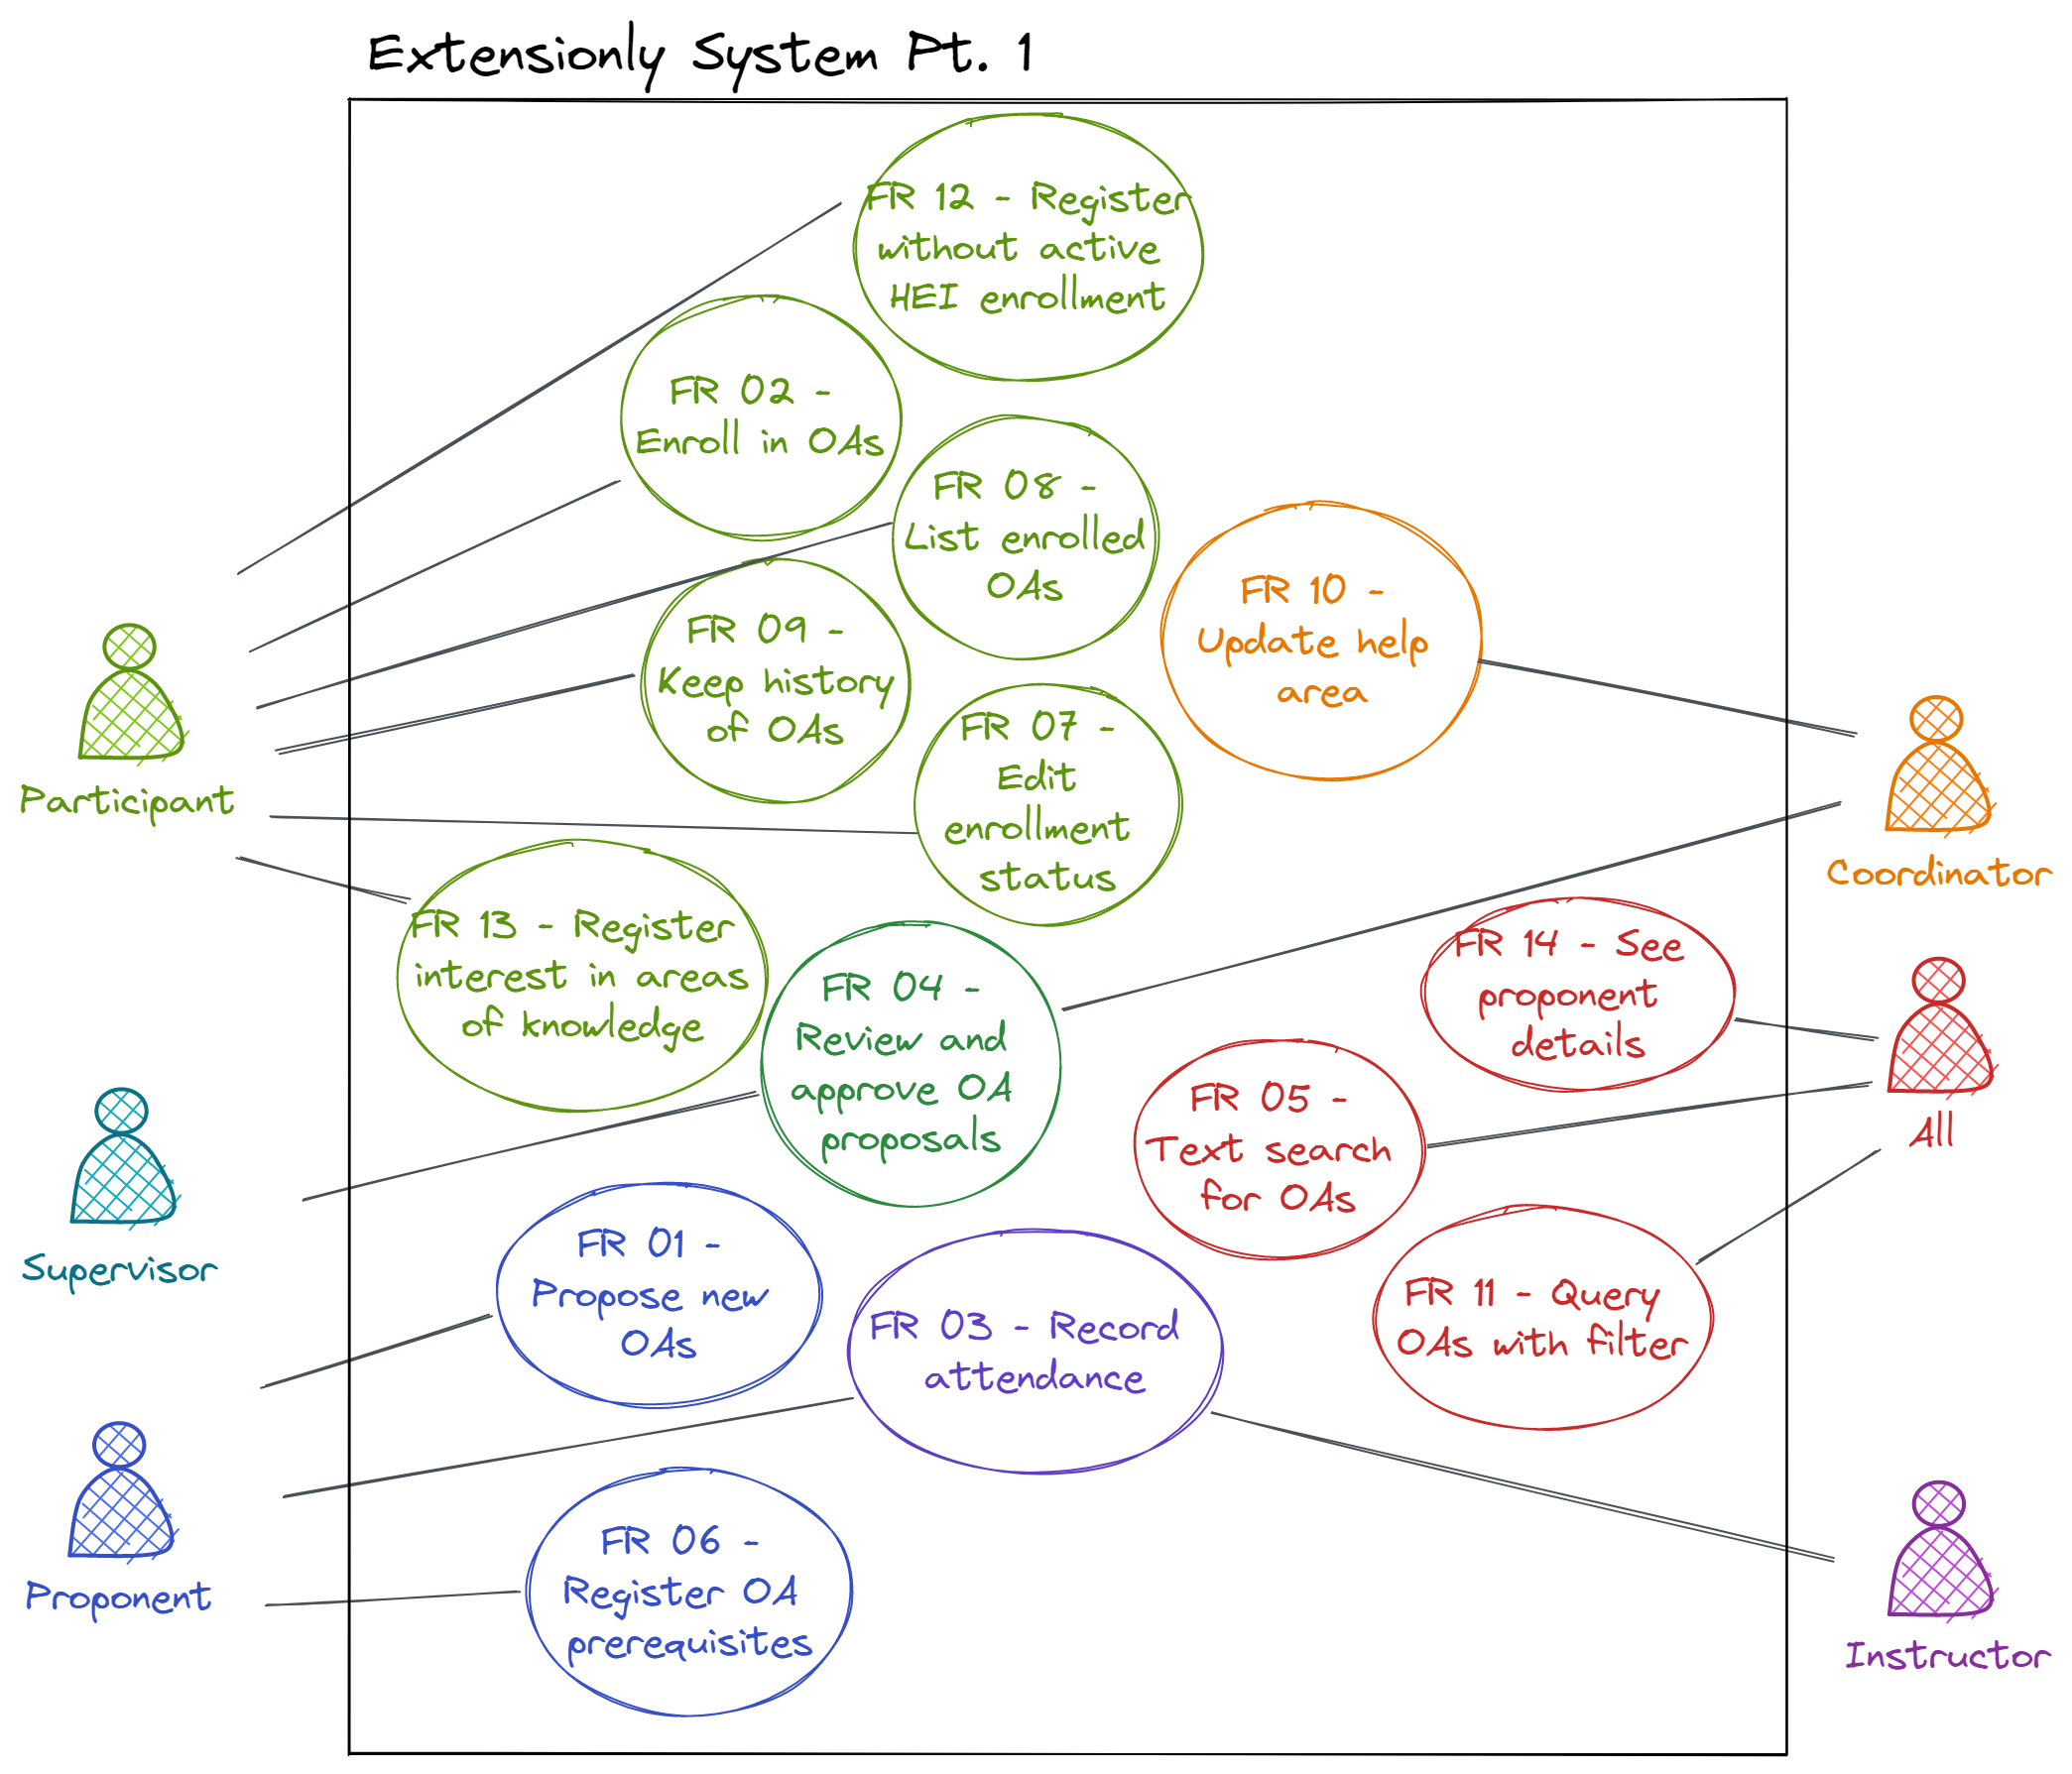
\includegraphics[width=15cm]{img/6-use-case-1.png}
  \end{center}
  \fonte{Author.}
\end{figure}

\begin{figure}[!htb]
  \caption{User Roles on the Last 8 \ac{FR}}\label{fig:use-case-2}
  \begin{center}
    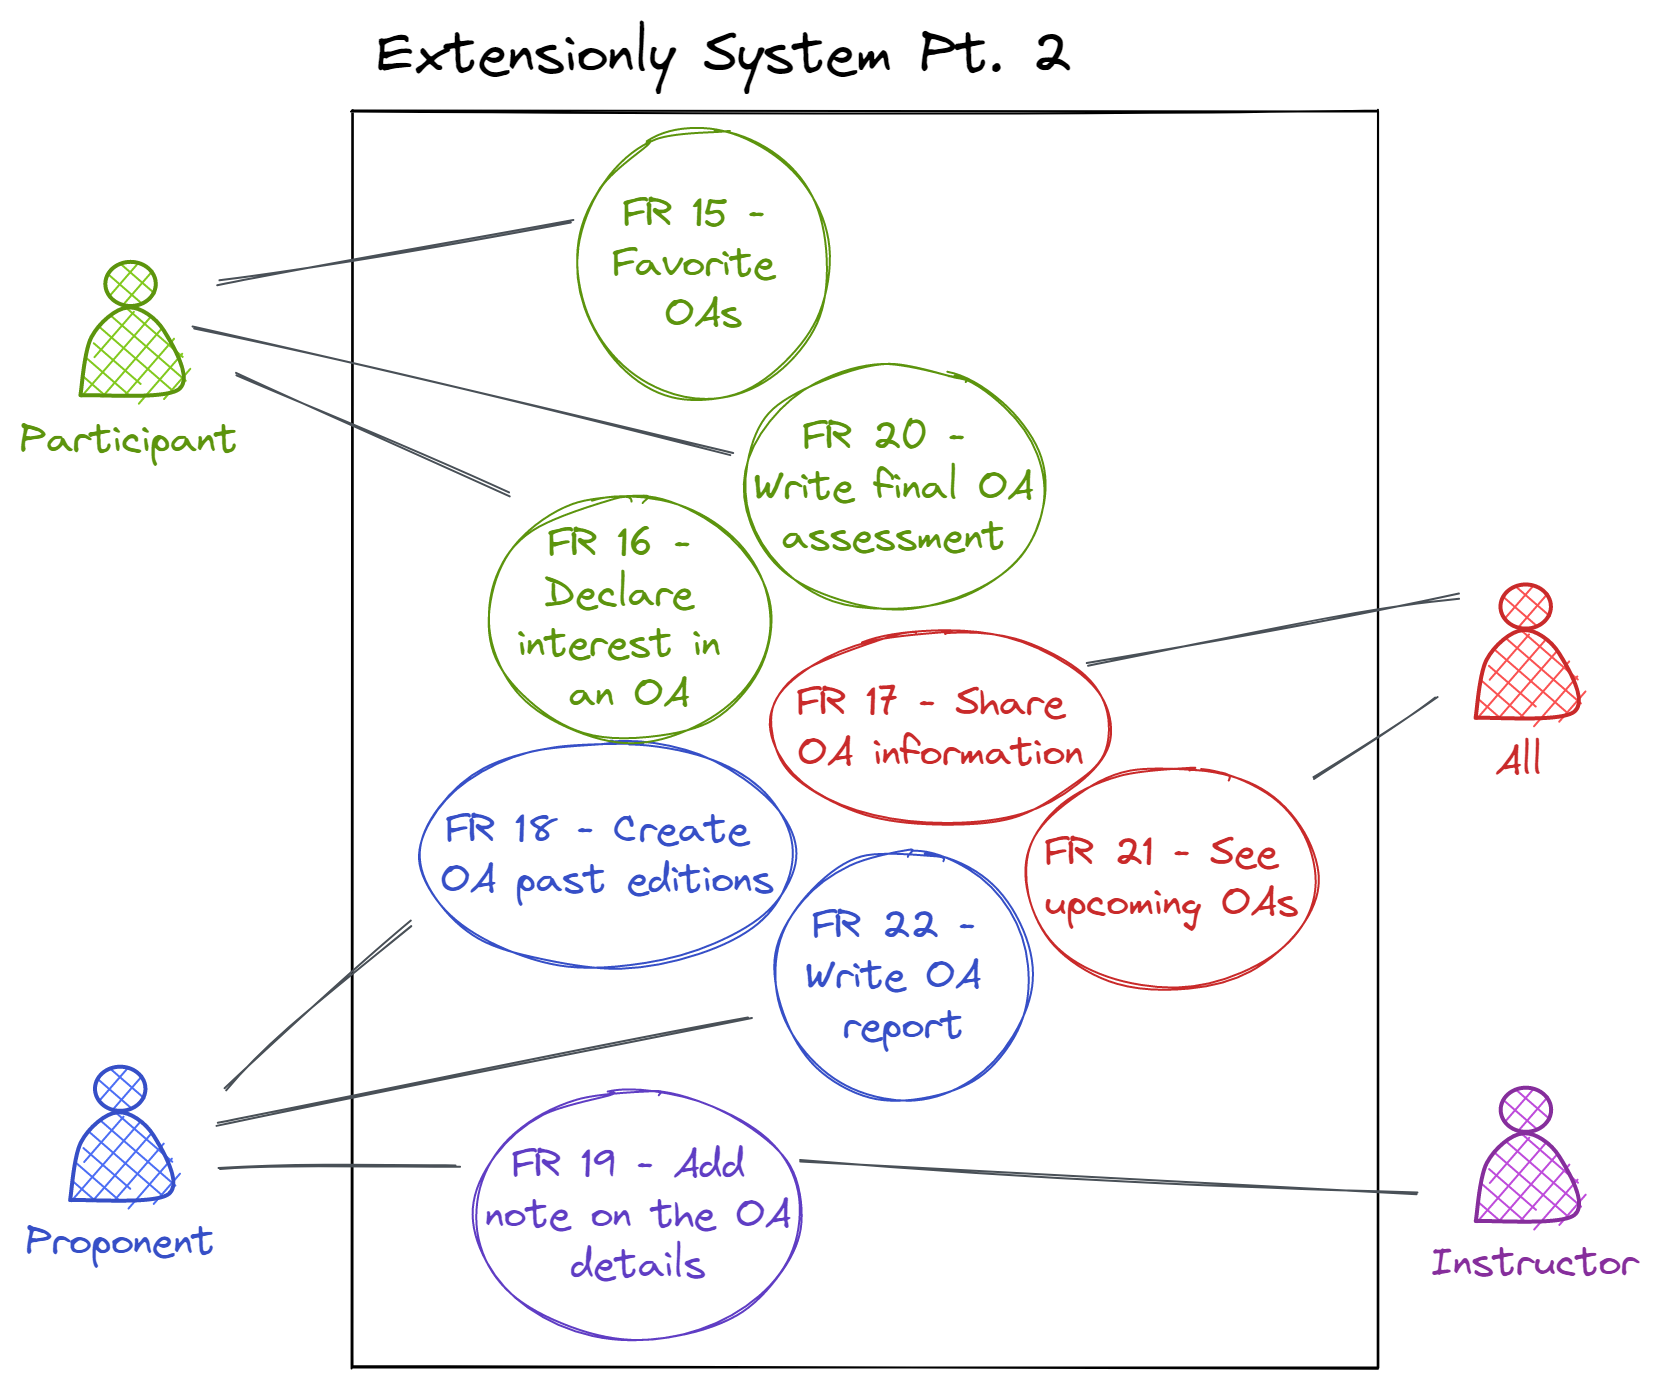
\includegraphics[width=12cm]{img/6-use-case-2.png}
  \end{center}
  \fonte{Author.}
\end{figure}

\subsection{User Stories derived from the Requirements}\label{ext:user-stories}

After the first round of defining the requirements, it was necessary to turn them into user stories, to use them in the survey, in a more descriptive form for the respondents. The stories were written with the system user roles in mind, which were presented earlier in \Cref{ext:initial-considerations}. They were used directly, with no other refinements, in the final survey and can be seen in \Cref{appendix:questionnaire}. However, in order to relate \acp{FR} with the questions and also update their ranking based on the survey results, \Cref{tab:stories-requirements-relation} was created:

\begin{table}[!htb]
  \centering
  \setlength{\aboverulesep}{0pt}
  \setlength{\belowrulesep}{0pt}
  \caption{User Stories}
  \label{tab:stories-requirements-relation}
  \footnotesize
  \begin{tabular}{c|c|c}
    \toprule
    \rowcolor[rgb]{0.753,0.753,0.753} \textbf{Requirement ID} & \textbf{Question/story ID} & \textbf{Priority} \\
    \hline
    \rowcolor[rgb]{0.898,0.898,0.898} FR. 01                  & P1                         & Must have         \\
    FR. 02                                                    & A1                         & Must have         \\
    \rowcolor[rgb]{0.898,0.898,0.898} FR. 03                  & I1                         & Must have         \\
    FR. 04                                                    & C1                         & Must have         \\
    \rowcolor[rgb]{0.898,0.898,0.898} FR. 05                  & A2                         & Must have         \\
    FR. 06                                                    & P2                         & Should have       \\
    \rowcolor[rgb]{0.898,0.898,0.898} FR. 07                  & A3                         & Must have         \\
    FR. 08                                                    & A5                         & Must have         \\
    \rowcolor[rgb]{0.898,0.898,0.898} FR. 09                  & A5                         & Must have         \\
    FR. 10                                                    & A6                         & Must have         \\
    \rowcolor[rgb]{0.898,0.898,0.898} FR. 11                  & A2                         & Must have         \\
    FR. 12                                                    & A11                        & Will not have     \\
    \rowcolor[rgb]{0.898,0.898,0.898} FR. 13                  & A8                         & Must have         \\
    FR. 14                                                    & P3                         & Should have       \\
    \rowcolor[rgb]{0.898,0.898,0.898} FR. 15                  & A9                         & Must have         \\
    FR. 16                                                    & A10                        & Must have         \\
    \rowcolor[rgb]{0.898,0.898,0.898} FR. 17                  & A12                        & Should have       \\
    FR. 18                                                    & P6                         & Must have         \\
    \rowcolor[rgb]{0.898,0.898,0.898} FR. 19                  & P4                         & Should have       \\
    FR. 20                                                    & A13                        & Should have       \\
    \rowcolor[rgb]{0.898,0.898,0.898} FR. 21                  & A14                        & Must have         \\
    FR. 22                                                    & P5                         & Should have       \\
    \bottomrule
  \end{tabular}
\end{table}

There were some cases where multiple \acp{FR} were assigned to a single user story, because the requirements are usually more technical, while a user story is supposed to have a higher level of abstraction.

% user stories used to write the survey questions
% new priority based on survey results

\section{Design Decisions}\label{ext:design-decisions}

The decisions made regarding the development of the goal product are discussed in this section.

\begin{description}
  \item[\textbf{Programming Language:}] \ac{TS} was chosen because of the incredible ecosystem of tools and technologies built around it. It expands the capabilities of common \ac{JS}, a dynamic typed language, by enforcing the usage of types in it. This makes it more strict, which increases robustness and predictiveness.
  \item[\textbf{Architecture:}] The architecture comes with the chosen framework the tool is being developed in: NextJS with React. The \ac{UI} is component based, meaning each element can be treated as an individual component, such as buttons and cards. It enables reusability, reducing duplicated code and in consequence, less convoluted applications. The website the user sees is a tree where each node is a component. The architecture can be seen in \Cref{fig:arch}.

    \begin{figure}[!htb]
      \caption{Front end Architecture}\label{fig:arch}
      \begin{center}
        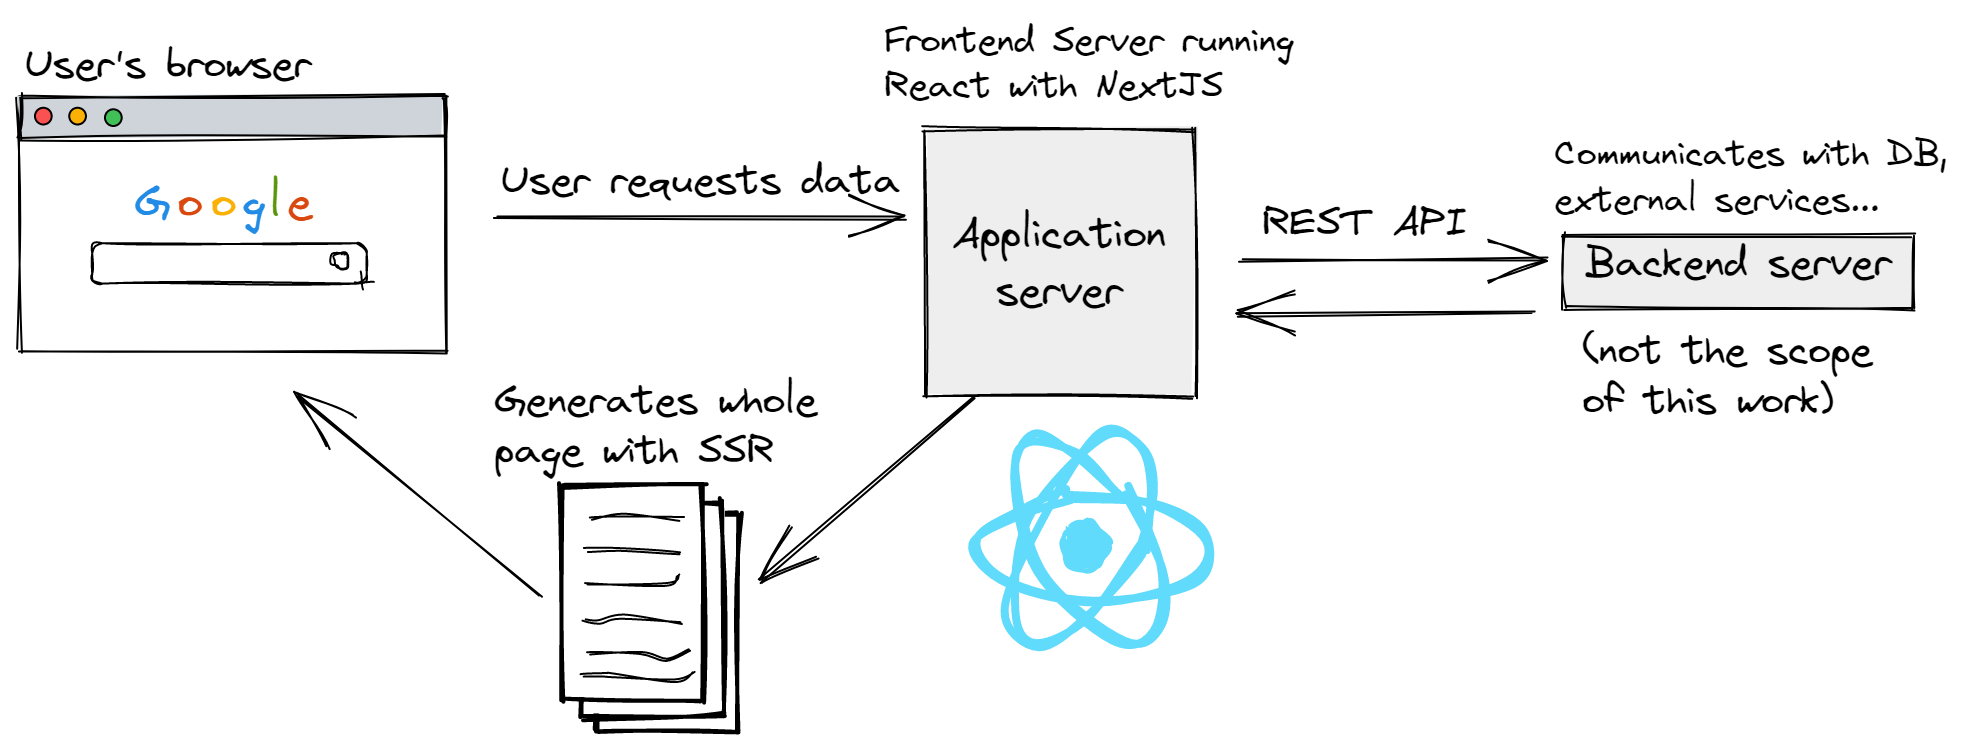
\includegraphics[width=14cm]{img/6-architecture.png}
      \end{center}
      \fonte{Author.}
    \end{figure}

    Regarding NextJS, it was chosen because of its \ac{SSR} capabilities. This greatly reduces loading times for the user, because the whole page document with its \ac{HTML} tags are pre generated on the application server and delivered all at once when the page loads. This is not normally the case for React applications, which rely on \ac{CSR}. With this approach, the React framework sends the bare minimum information needed in the first load, followed by a loading spinner to the user while the page itself is generated locally in the user's browser. \Cref{fig:ssr} and \Cref{fig:csr} aim to illustrate this behavior.

    \begin{figure}[!htb]
      \caption{\acl{CSR}}\label{fig:csr}
      \begin{center}
        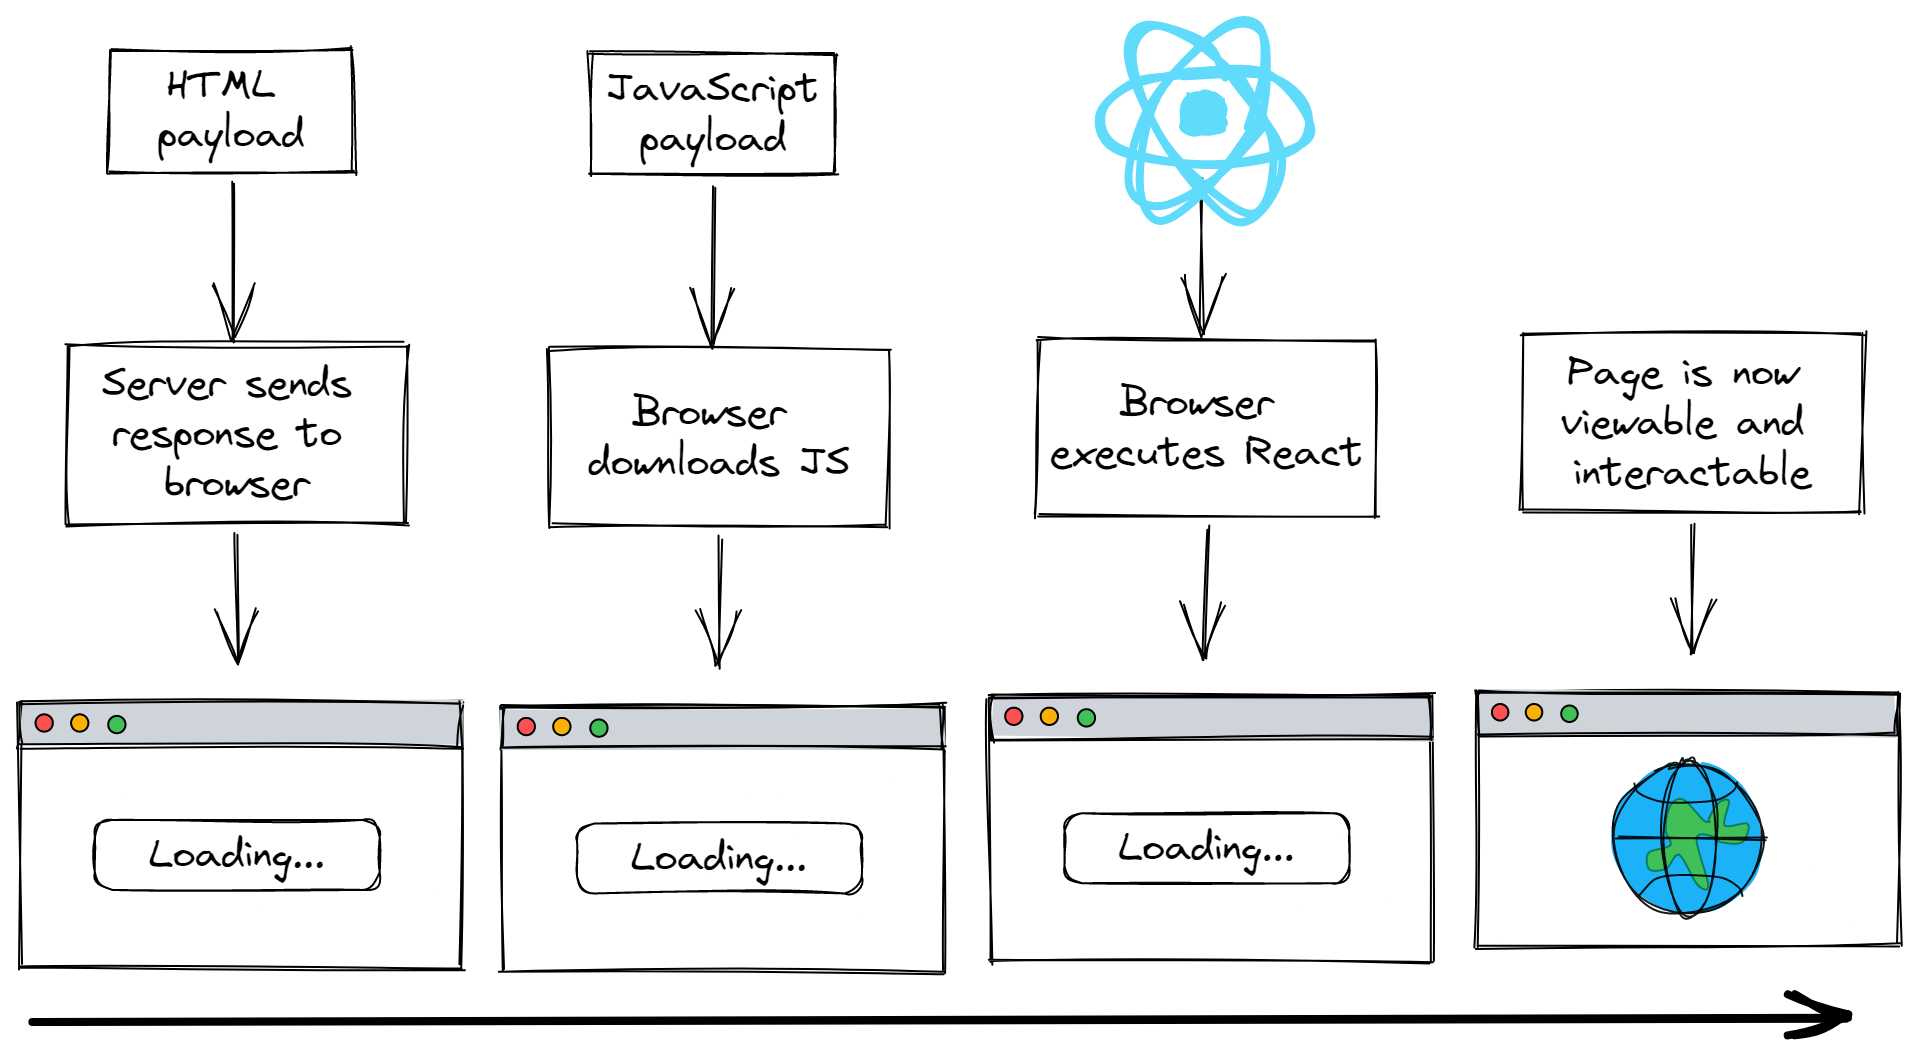
\includegraphics[width=14cm]{img/6-csr.png}
      \end{center}
      \fonte{Author.}
    \end{figure}

    \begin{figure}[!htb]
      \caption{\acl{SSR}}\label{fig:ssr}
      \begin{center}
        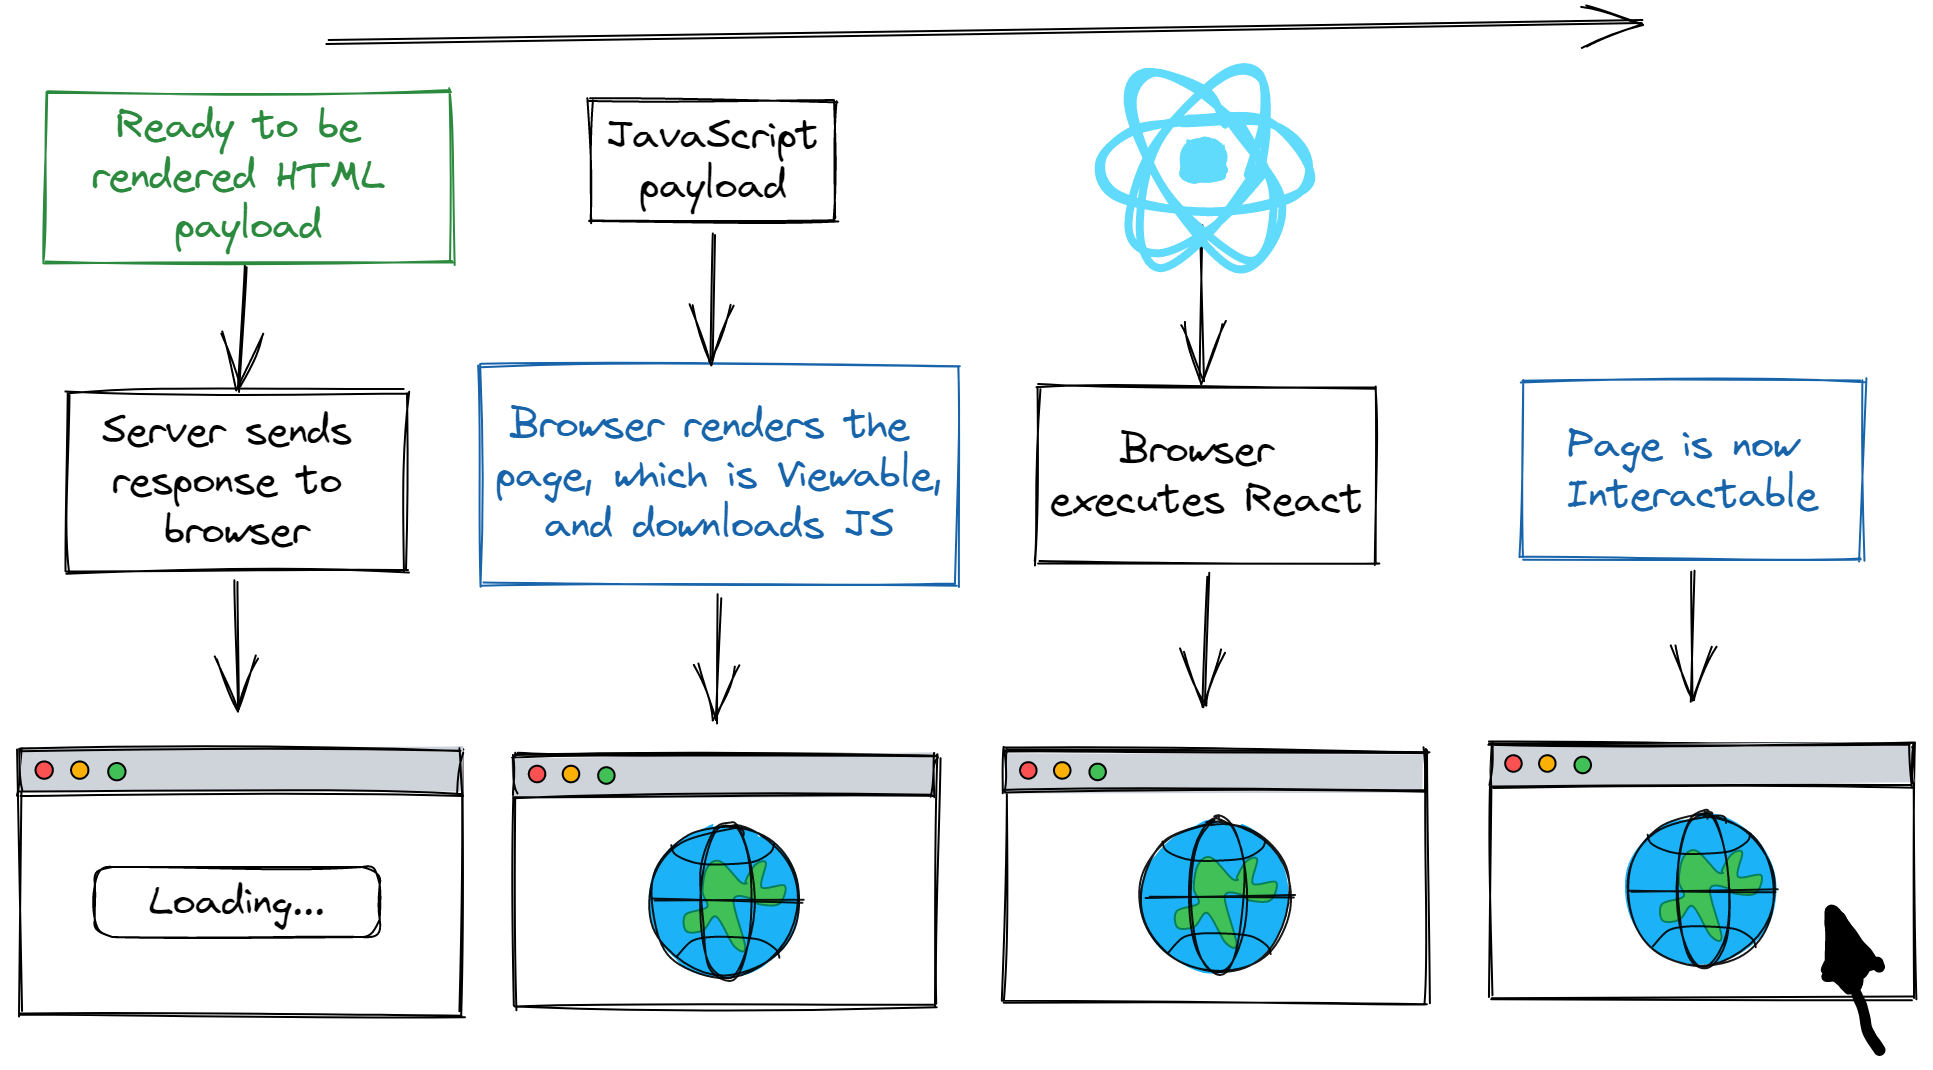
\includegraphics[width=14cm]{img/6-ssr.png}
      \end{center}
      \fonte{Author.}
    \end{figure}
  \item[\textbf{License:}] The front end web application is licensed under the GNU General Public License v3.0, which is an open source license and is very permissive, allowing even for commercial use. It does not provider however, any kind of warranty or liability regarding the software \cite{gnugpl3}.

\end{description}
